\documentclass[aspectratio=169]{beamer}
\usepackage[utf8]{inputenc}
\usepackage{amsmath}
\usepackage{tikz}
\usepackage{dsfont}
\usepackage{opensans}

\usetheme{NOVASBE}

\title[]{4509 - Bridging Mathematics}
\subtitle{Matrices}
\author[P. Fagandini]{Paulo Fagandini}
\institute{}
\date{}

\newtheorem{proposition}{Conjecture}[section]

\begin{document}

\begin{frame}{Introduction}
    \begin{center}
        \begin{tikzpicture}[scale=0.6,every node/.style = {scale = 0.6}]
            \draw[<->,thick] (-5,0) -- (5,0);
            \draw[<->,thick] (0,-3) -- (0,5);
            
            \onslide<2->{
                \draw[->,thick,orange] (0,0) -- (-2,1)node[left]{$v$};
            }
        
            \onslide<3->{
                \draw[->,red] (0,0) -- (1,0)node[below]{\(\hat{\imath}\)};
                \draw[->,blue] (0,0) -- (0,1)node[right]{\(\hat{\jmath}\)};
            }
            
        \end{tikzpicture}
        \onslide<2>{\[v=\begin{bmatrix}-2\\1\end{bmatrix}\]}
        \onslide<3>{\[v=-2\times\hat{\imath}+1\times\hat{\jmath}=-2\times\begin{bmatrix}1\\0\end{bmatrix}+1\times\begin{bmatrix}0\\1\end{bmatrix}=\begin{bmatrix}-2\\1\end{bmatrix}\]}
    \end{center}
\end{frame}

\begin{frame}{Introduction}
    Being not very rigorous, we can define a linear transformation as a transformation on every vector on the plane that must satisfy 2 things:
    \begin{enumerate}
        \item Lines must be transformed into lines
        \item The origin must remain in the same place
    \end{enumerate}
    We will deal with the formal definition and rigor later...
    
\end{frame}

\begin{frame}{Introduction}
    \begin{columns}        
        \begin{column}{0.5\textwidth}
            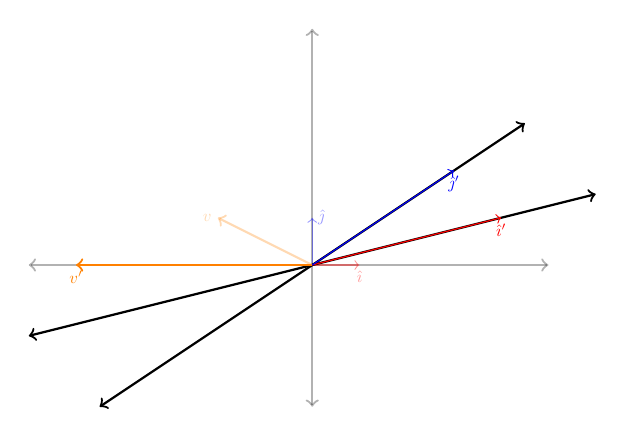
\begin{tikzpicture}[scale=0.6,every node/.style = {scale = 0.6}]
                \draw[<->,thick,opacity=0.3] (-6,0) -- (5,0);
                \draw[<->,thick,opacity=0.3] (0,-3) -- (0,5);
                \draw[->,thick,orange,opacity=0.3] (0,0) -- (-2,1)node[left]{$v$};
                
                \draw[->,red,opacity=0.4] (0,0) -- (1,0)node[below]{\(\hat{\imath}\)};
                \draw[->,blue,opacity=0.4] (0,0) -- (0,1)node[right]{\(\hat{\jmath}\)};
                
                \draw[<->,thick] (-6,-1.5) -- (6,1.5);
                \draw[<->,thick] (-4.5,-3) -- (4.5,3);
    
                \onslide<1->{
                    \draw[->,red] (0,0) -- (4,1)node[below]{\(\hat{\imath}'\)};
                    \draw[->,blue] (0,0) -- (3,2)node[below]{\(\hat{\jmath}'\)};
                }
                
                \onslide<4->{
                    \draw[->,thick,orange] (0,0) -- (-5,0)node[below]{$v'$};
                }
                
            \end{tikzpicture}
        \end{column}
        \begin{column}{0.5\textwidth}
            {\small
            \only<2>{\[\hat{\imath}'=\begin{bmatrix}4\\1\end{bmatrix}\quad\hat{\jmath}'=\begin{bmatrix}3\\2\end{bmatrix}\]}
            \only<3>{\[v=-2\times\hat{\imath}'+1\times\hat{\jmath}'=-2\times\begin{bmatrix}4\\1\end{bmatrix}+1\times\begin{bmatrix}3\\2\end{bmatrix}=\begin{bmatrix}-5\\0\end{bmatrix}\]}
            \only<5>{\[w=\begin{bmatrix}x\\y\end{bmatrix} \text{ lands on } x\times \begin{bmatrix}4\\1\end{bmatrix}+y\times \begin{bmatrix}3\\2\end{bmatrix}=\begin{bmatrix}4x+3y\\1x+2y\end{bmatrix}\]}
            \only<6>{\[\begin{bmatrix}1&0\\0&1\end{bmatrix}\begin{bmatrix}x\\y\end{bmatrix}=\begin{bmatrix}x\\y\end{bmatrix}=x\times \hat{\imath}+y\times \hat{\jmath}\]
            \[\begin{bmatrix}4&3\\1&2\end{bmatrix}\begin{bmatrix}x\\y\end{bmatrix}=\begin{bmatrix}4x+3y\\1x+2y\end{bmatrix}=x\times\hat{\imath}'+y\times\hat{\jmath}'\]}
            }
        \end{column}
    \end{columns}
\end{frame}

\begin{frame}{Introduction}
    What about another vector in the same ``direction'' than $v$? say \[z=\begin{bmatrix}1\\-0.5\end{bmatrix}\] ... \pause
    
    \[\begin{bmatrix}4&3\\1&2\end{bmatrix}\begin{bmatrix}1\\-0.5\end{bmatrix}=\begin{bmatrix}2.5\\0\end{bmatrix}\]
\end{frame}

\begin{frame}{Introduction}
    \begin{center}
        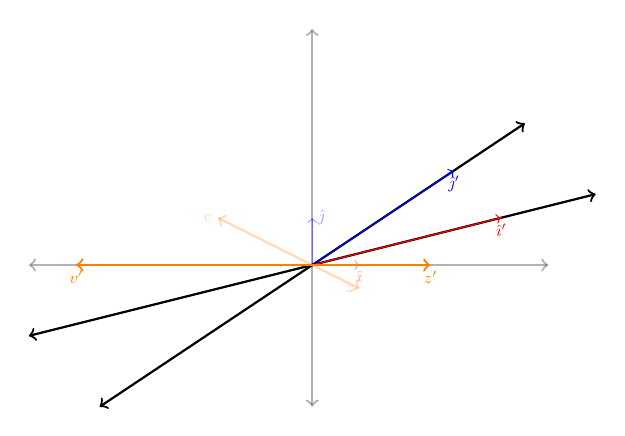
\begin{tikzpicture}[scale=0.6,every node/.style = {scale = 0.6}]
            \draw[<->,thick,opacity=0.3] (-6,0) -- (5,0);
            \draw[<->,thick,opacity=0.3] (0,-3) -- (0,5);
            \draw[->,thick,orange,opacity=0.3] (0,0) -- (-2,1)node[left]{$v$};
            \draw[->,thick,orange,opacity=0.3] (0,0) -- (1,-0.5)node[left]{$z$};
            
            \draw[->,red,opacity=0.4] (0,0) -- (1,0)node[below]{\(\hat{\imath}\)};
            \draw[->,blue,opacity=0.4] (0,0) -- (0,1)node[right]{\(\hat{\jmath}\)};
            
            \draw[<->,thick] (-6,-1.5) -- (6,1.5);
            \draw[<->,thick] (-4.5,-3) -- (4.5,3);

            \onslide<1->{
                \draw[->,red] (0,0) -- (4,1)node[below]{\(\hat{\imath}'\)};
                \draw[->,blue] (0,0) -- (3,2)node[below]{\(\hat{\jmath}'\)};
            }
            
            \onslide<1->{
                \draw[->,thick,orange] (0,0) -- (2.5,0)node[below]{$z'$};
                \draw[->,thick,orange] (0,0) -- (-5,0)node[below]{$v'$};
            }
            
        \end{tikzpicture}
    \end{center}
\end{frame}

\begin{frame}{Introduction}
    So transforming two vectors in the same line, they both end up also in the same line... keep this in mind.
\end{frame}

\begin{frame}{Introduction}
    Could we take back $\hat{\imath}'$ to $\hat{\imath}$ and $\hat{\jmath}'$ to $\hat{\jmath}$? \pause
    
    Sure, if we apply the transform \[\begin{bmatrix}0.4&-0.6\\-0.2&0.8\end{bmatrix}\] \pause
    
    \[\begin{bmatrix}0.4&-0.6\\-0.2&0.8\end{bmatrix}\begin{bmatrix}4&3\\1&2\end{bmatrix}=\begin{bmatrix}1&0\\0&1\end{bmatrix}\]
    
    Applying the inverse!
\end{frame}

\begin{frame}{Introduction}
    The important thing is that: if the vectors are linearly dependent, then we cannot invert the matrix, we just saw that two vectors that reside on the same line, end up in the same (although probably a different one) line.
\end{frame}

\begin{frame}{Introduction}
    There are a couple of interesting vectors on the whole space when we apply this linear transformation...
    
    Take for example the following vector:\(e=\begin{bmatrix}-1\\1\end{bmatrix}\)\pause
    \[\begin{bmatrix}4&3\\1&2\end{bmatrix}\begin{bmatrix}-1\\1\end{bmatrix}=\begin{bmatrix}-1\\1\end{bmatrix}\]
\end{frame}

\begin{frame}{Introduction}
    \begin{center}
        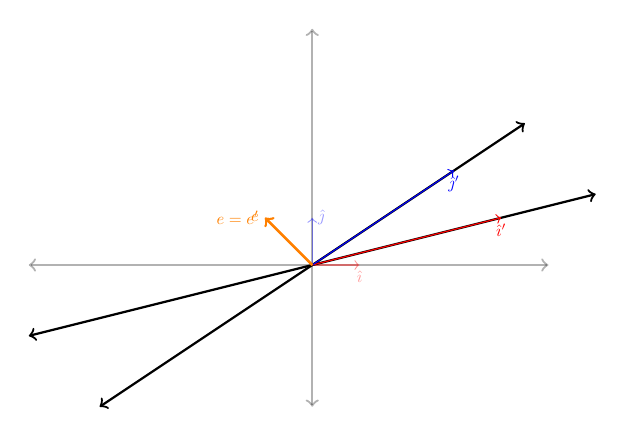
\begin{tikzpicture}[scale=0.6,every node/.style = {scale = 0.6}]
            \draw[<->,thick,opacity=0.3] (-6,0) -- (5,0);
            \draw[<->,thick,opacity=0.3] (0,-3) -- (0,5);

            \draw[->,red,opacity=0.4] (0,0) -- (1,0)node[below]{\(\hat{\imath}\)};
            \draw[->,blue,opacity=0.4] (0,0) -- (0,1)node[right]{\(\hat{\jmath}\)};
            
            \draw[<->,thick] (-6,-1.5) -- (6,1.5);
            \draw[<->,thick] (-4.5,-3) -- (4.5,3);

            \onslide<1->{
                \draw[->,red] (0,0) -- (4,1)node[below]{\(\hat{\imath}'\)};
                \draw[->,blue] (0,0) -- (3,2)node[below]{\(\hat{\jmath}'\)};
            }
            \onslide<1>{
                \draw[->,orange,thick](0,0)--(-1,1)node[left]{\(e\)};
            }
            
            \onslide<2>{
                \draw[->,orange,thick](0,0)--(-1,1)node[left]{\(e=e'\)};
            }
            
        \end{tikzpicture}
        \only<2>{
            \[
            \begin{bmatrix}
                1&0\\0&1
            \end{bmatrix}
            \begin{bmatrix}
                -1\\1
            \end{bmatrix}=\begin{bmatrix}
                -1\\1
            \end{bmatrix}=
            \begin{bmatrix}
                4&3\\1&2
            \end{bmatrix}
            \begin{bmatrix}
                -1\\1
            \end{bmatrix}\]
            }
            \only<3>{\[e.v._1=\begin{bmatrix}-1,1\end{bmatrix},\quad \lambda_1=1\]}
    \end{center}
\end{frame}

\begin{frame}{Introduction}

    Or the vector:\(f=\begin{bmatrix}0.9487\\0.3162\end{bmatrix}\)\pause
    \[\begin{bmatrix}4&3\\1&2\end{bmatrix}\begin{bmatrix}0.9487\\0.3162\end{bmatrix}=\begin{bmatrix}4.7434\\1.5811\end{bmatrix}\]
    
\end{frame}

\begin{frame}{Introduction}
    \begin{center}
        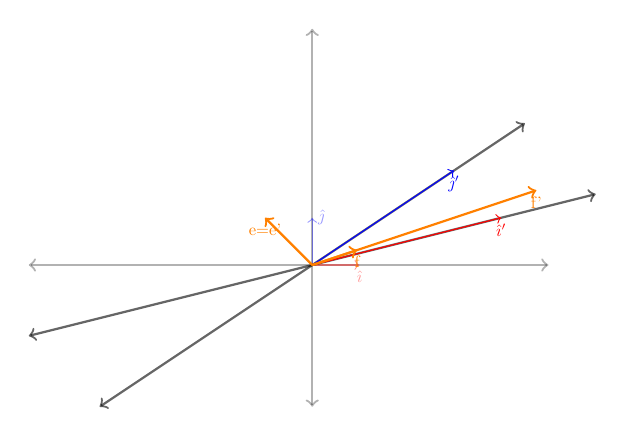
\begin{tikzpicture}[scale=0.6,every node/.style = {scale = 0.6}]
            \draw[<->,thick,opacity=0.3] (-6,0) -- (5,0);
            \draw[<->,thick,opacity=0.3] (0,-3) -- (0,5);

            \draw[->,red,opacity=0.4] (0,0) -- (1,0)node[below]{\(\hat{\imath}\)};
            \draw[->,blue,opacity=0.4] (0,0) -- (0,1)node[right]{\(\hat{\jmath}\)};
            
            \draw[<->,thick,opacity=0.6] (-6,-1.5) -- (6,1.5);
            \draw[<->,thick,opacity=0.6] (-4.5,-3) -- (4.5,3);

            \onslide<1->{
                \draw[->,red] (0,0) -- (4,1)node[below]{\(\hat{\imath}'\)};
                \draw[->,blue] (0,0) -- (3,2)node[below]{\(\hat{\jmath}'\)};
                \draw[->,orange,thick](0,0)--(-1,1)node[below]{e=e'};
                \draw[->,orange,thick](0,0)--(0.9487,0.3162)node[below]{f};
            }
            
            \onslide<2>{
                \draw[->,orange,thick](0,0)--(4.7434,1.5811)node[below]{f'};
            }
            
        \end{tikzpicture}
        \only<2>{
            \[
            5\times
            \begin{bmatrix}
                1&0\\0&1
            \end{bmatrix}
            \begin{bmatrix}
                0.9487\\0.3162
            \end{bmatrix}=\begin{bmatrix}
                4.7434\\1.5811
            \end{bmatrix}=
            \begin{bmatrix}
                4&3\\1&2
            \end{bmatrix}
            \begin{bmatrix}
                0.9487\\0.3162
            \end{bmatrix}\]
            }
            \only<3>{\[e.v._2=\begin{bmatrix}0.9487\\0.3162\end{bmatrix},\quad \lambda_2=5\]}
    \end{center}
\end{frame}

\begin{frame}{Introduction}
    What happens with these vectors?
    
    \begin{table}[]
        \centering
        \renewcommand{\arraystretch}{1.5}
        \begin{tabular}{ccc}
            & \(ev_1\) & \(ev_2\)\\\hline
            \(A\times\) & \(\begin{bmatrix}-1\\1\end{bmatrix}\) & \(\begin{bmatrix}4.7434\\1.5811\end{bmatrix}\) \\
            \onslide<2->{\(A^2\times\) & \(\begin{bmatrix}-1\\1\end{bmatrix}\) & \(\begin{bmatrix}23.7171\\7.9057\end{bmatrix}\)  }\\
            \onslide<3->{\(A^3\times\) & \(\begin{bmatrix}-1\\1\end{bmatrix}\) & \(\begin{bmatrix}118.585\\39.528\end{bmatrix}\)} \\\hline
            \onslide<4->{\(\lambda\) & 1 & 5}
        \end{tabular}
    \end{table}
    
\end{frame}

\begin{frame}
    \begin{definition}
        A real \textbf{matrix} is a rectangular array of real numbers.
        
        \begin{align*}
            A = \left(
            \begin{array}{cccc}
                a_{11} & a_{12} & \ldots & a_{1n}\\
                a_{21} & a_{22} & \ldots & a_{2n}\\
                \vdots & \vdots & \ddots & \vdots \\
                a_{m1} & a_{m2} & \ldots & a_{nm} 
            \end{array}
            \right)
        \end{align*}
        
        Where $a_{ij}\in\mathds{R}$. $A$ is said to be an element of $\mathds{R}^{m\times n}$
    \end{definition}
    
    A vector would be then a matrix with only 1 column!
\end{frame}

\begin{frame}
    Let $A,B\in\mathds{R}^{m\times n}$. Let $C\in\mathds{R}^{n\times l}$. Finally, let $\alpha\in\mathds{R}$.
    \begin{enumerate}
        \item $[A+B]_{ij} = a_{ij}+b_{ij}$
        \item $[A \cdot C]_{ik}=\sum_{j=1}^n a_{ij}\cdot c_{jk}$, and it has a dimension $m\times l$
        \item $[\alpha A]_{ij}=\alpha a_{ij}$
    \end{enumerate}
\end{frame}

\begin{frame}
    \begin{definition}
        Let $A\in\mathds{R}^{m\times n}$, $A$'s \textbf{transpose}, denoted $A^t\in\mathds{R}^{n\times m}$ is such that its elements are:
        
        \begin{align*}
            a^t_{ij}=a_{ji}
        \end{align*}
    \end{definition}
    
    \begin{definition}
        Matrix $A\in\mathds{R}^{m\times n}$ is said to be \textbf{squared} if $n=m$
    \end{definition}
    
    \begin{definition}
        Matrix $A$ is said to be \textbf{symmetric} if $A^t=A$
    \end{definition}
    \begin{definition}
        Matrix $A$ is said to be \textbf{antisymmetric} if $A^t=-A$
    \end{definition}
\end{frame}

\begin{frame}
    \begin{definition}
        The \textbf{Identity} is a squared matrix $I_n\in\mathds{R}^{n\times n}$ that has $I_{ij}=0$ if $i\neq j$, and $I_{ij}=1$ if $i=j$.
    \end{definition}
    
    The identity has a nice property: $A I_n = I_m A= A$ for any $A\in\mathds{R}^{m\times n}$.
    
    \begin{definition}
        Matrix $A$ is \textbf{invertible}, if there is another matrix $A^{-1}$ such that $A\cdot A^{-1} = A^{-1}\cdot A = I$
    \end{definition}
\end{frame}

\begin{frame}
    \begin{proposition}
        Given $A,B,C\in\mathds{R}^{n\times n}$
        
        \begin{enumerate}
            \item $A+B=B+A$
            \item $A(BC)=(AB)C$
            \item $A(B+C)=AB+AC$
            \item $(A+B)^t = A^t+B^t$
            \item $(AB)^t=B^tA^t$
            \item $(A^t)^t=A$
            \item If $A$ and $B$ are invertible, then $AB$ and $BA$ are invertible as well. Furthermore $(AB)^{-1}=B^{-1}A^{-1}$
            \item If $A$ is invertible, then $(A^t)^{-1}=(A^{-1})^t$
        \end{enumerate}
    \end{proposition}
\end{frame}

\begin{frame}
    Quick quiz, 15 min, prove points 7 and 8. You can use points 1-6 as true and given.
\end{frame}

\begin{frame}{Solution}
    \begin{enumerate}
    
    \item[7] Start with $AB$, multiply by $A^{-1}$ from the left, you are left with $A^{-1}AB = Id B = B$. Now multiply by $B^{-1}$, so you get $B^{-1}A^{-1}AB = B^{-1}IdB=B^{-1}B=Id$. Then $(B^{-1}A^{-1})(AB) = Id$ so it must be that $B^{-1}A^{-1}=(AB)^{-1}$. To complete the proof, you need to show that you can do the same from the ``right''.
    
    \item[8] Start with $(A^{-1}A)^t = Id ^t = Id$, use property 5 and you get $(A^{-1}A)^t = A^t (A^{-1})^t = Id$, then $(A^{-1})^t$ must be the inverse (again the only thing that is missing is to show that it works if you start with $(A A^{-1})^t$ as well which is trivial.
    
    \end{enumerate}
\end{frame}

\begin{frame}
\begin{proposition}
    The set of the matrices in $\mathds{R}^{m\times n}$, together with the sum and scalar multiplication is a vector space.    
\end{proposition}

\begin{proposition}
A squared matrix $A\in\mathds{R}^{n\times n}$ is invertible if and only if all of its columns are linearly independent.
\end{proposition}
\end{frame}


\begin{frame}
    \begin{definition}
        Matrix $A\in\mathds{R}^{m\times n}$ is \textbf{upper triangular} if it has the following shape:
        
        \begin{align*}
            A=\left[
            \begin{array}{cccccc}
                a_{11} & a_{12} & \ldots & a_{1m} & \ldots & a_{1n}\\
                0 & a_{22} & \ldots & a_{2m} & \ldots & a_{2n}\\
                0 & 0 & \ddots & \vdots & \ldots& \vdots\\
                0 & 0 & \ldots & a_{mm} & \ldots & a_{mn}
            \end{array}
            \right]
        \end{align*}
        
        That is, it has zeroes below its main diagonal.
    \end{definition}
    
    \begin{proposition}
        The set of the upper triangular matrices in $\mathds{R}^{n\times m}$, with the sum and scalar multiplication is a vector subspace of $\mathds{R}^{n\times m}$.
    \end{proposition}
\end{frame}

\begin{frame}
    \begin{definition}
        Matrix $A$ is \textbf{lower triangular} if $A^t$ is upper triangular.
    \end{definition}

    \begin{definition}
        Matrix $A$ is \textbf{diagonal} if it is upper and lower triangular at the same time.
    \end{definition}

    \begin{definition}
        The \textbf{rank} of a matrix $A$, denoted by $rank(A)$ is the maximum number of linearly independent rows or columns of $A$.
    \end{definition}
\end{frame}

\begin{frame}
    A convenient way to write down a system of equations:
    \begin{align*}
        \begin{array}{ccccccccc}
        a_{11} x_1 &+& a_{12} x_2 &+&\ldots &+& a_{1n}x_n  &=& b_1\\
        a_{21} x_1 &+& a_{22} x_2 &+&\ldots &+& a_{1n}x_n  &=& b_2\\
        \vdots & &  \vdots & &\ldots & & \vdots  & & \vdots\\
        a_{m1} x_1 &+& a_{m2} x_2 &+&\ldots &+& a_{mn}x_n  &=& b_m
        \end{array}
    \end{align*}
    
    It would be $A X = B$, where,
    \begin{align*}
        A=\left(\begin{array}{ccc}a_{11}&\ldots&a_{1n}\\ \vdots & \ddots & \vdots \\ a_{m1}&\ldots&a_{mn}\end{array}\right)\quad X=\left(\begin{array}{c}x_1\\ \vdots \\ x_n\end{array}\right) \quad
        B = \left(\begin{array}{c}
             b_1\\\vdots \\ b_m
        \end{array}\right)
    \end{align*}
\end{frame}

\begin{frame}
\begin{definition}
    Given a system of equations $AX=B$, \begin{itemize}
        \item $\hat{X}\in\mathds{R}^n$ is a \textbf{particular solution} of the system if $A\hat{X}=B$.
        \item $X_0$ is an \textbf{homogeneous solution} if $AX_0=0$.
    \end{itemize}
    
    
\end{definition}
    
    Note that for $\lambda\in\mathds{R}$, $A(\hat{X}+\lambda X_0)=A\hat{X}+\lambda A X_0 = B+0 = B$.
    
    \vspace{0.5cm}
    
\end{frame}

\begin{frame}
    \begin{definition}
        The \textbf{kernel} of $A\in\mathds{R}^{m\times n}$ is defined as:
        \begin{align*}
            Ker(A):=\{X\in\mathds{R}^n| AX = 0\}
        \end{align*}
    \end{definition}
    
    \begin{proposition}
        $Ker(A)\subseteq\mathds{R}^n$ is a vector subspace of $\mathds{R}^n$
    \end{proposition}
    
    \begin{definition}
        The dimension of $Ker(A)$ is called the \textbf{nullity} --- or nullspace ---, and it is denoted by $Null(A)$. If $Ker(A)=\{0\}$, then $Null(A)=0$.
    \end{definition}
    
    Note that a system of equations as the one shown before, has unique solution only if $Null(A)=0$.
    
\end{frame}

\begin{frame}
    \begin{proposition}
        Matrix $A\in\mathds{R}^{n\times n}$ is invertible if and only if $Null(A)=0$.
    \end{proposition}
    
    \begin{proposition}
        $A\in\mathds{R}^{n\times n}$ is invertible if and only if the system $AX=B$ as a unique solution, for any $B\in\mathds{R}^n$.
    \end{proposition}
    
\end{frame}

\begin{frame}
    \begin{definition}
        The \textbf{image} of $A\in\mathds{R}^{n\times n}$ is defined as:
        \begin{align*}
            Im(A):=\{Y\in\mathds{R}^n|\exists X\in\mathds{R}^n, Y=AX\}\equiv \{AX|X\in\mathds{R}^n\}
        \end{align*}
    \end{definition}
    
    \begin{proposition}
        Let $A\in\mathds{R}^{n\times n}$. $Im(A)$ is a vector subspace of $\mathds{R}^n$.
    \end{proposition}
    
    \begin{definition}
        The dimension of $Im(A)$ is called the \textbf{range} of $A$. Let's denote it as $R(A)$.
    \end{definition}
\end{frame}

\begin{frame}
    \begin{proposition}
        Let $A\in\mathds{R}^{n\times n}$. $R(A)$ is the number of l.i. columns of $A$.
    \end{proposition}
    
    \begin{proposition}
        Consider $A\in\mathds{R}^{n\times n}$. It holds that $Null(A)+R(A)=n$.
    \end{proposition}
\end{frame}
\iffalse
\begin{frame}
    \begin{proposition}
        For any $A\in\mathds{R}^{n\times n}$, there is an invertible matrix $C$, and an upper triangular matrix $R$ such that, $$CA=R\Leftrightarrow A=C^{-1}R$$
    \end{proposition}
\end{frame}
\fi
\begin{frame}
    \begin{definition}
        The quadratic form associated to $A$ is a function $Q_A:\mathds{R}^n\rightarrow\mathds{R}$ such that for any $X\in\mathds{R}^n$,
        
        $$Q_A(X)=X^tAX\in\mathds{R}$$
    \end{definition}
\end{frame}

\begin{frame}

\begin{proposition}
    For any matrix $A\in\mathds{R}^{n\times n}$, there are always symmetric and antisymmetric matrices $S$ and $T$ such that $$A=S+T$$
\end{proposition}

Note:  Let $S=\frac{A+A^t}{2}$ and $T=\frac{A-A^t}{2}$. While $S$ is symmetric, $T$ is antisymmetric,
    
    
    \begin{corollary}
        A quadratic form can be represented as $$Q_A(X)=X^t S X$$ with $S$ symmetric.
    \end{corollary}
\end{frame}

\begin{frame}
    Quick quiz! 15 min to prove the corollary.
\end{frame}

\begin{frame}{Solution}
    
    \begin{itemize}
        \item Let $A = (S+T)$
        \item Then $Q_A(X) = X^t(S+T)X = X^tSX + X^tTX$
        \item But $X^tTX\in \mathds{R}$, so $(X^tTX)^t=X^tTX$ (a number trasposed is the same number).
        \item So you end up that $X^tTX = (X^tTX)^t = X^tT^tX$
        \item But $T$ is anytsymmetric so $T^t = -T$...
        \item Then $X^tTX = -X^tTX$, so if $X^tTX$ is the number $z$, you have $z=-z$, that only is true for $z=0$.
        \item Then $Q_A(X) = X^tSX$
    \end{itemize}
    
\end{frame}

\begin{frame}
    \begin{definition}
        Let $A\in\mathds{R}^{n\times n}$, symmetric. Consider the quadratic form $Q_A(X)=X^t A X$. If for any $X\in\mathds{R}^n\setminus\{0\}$,
        \begin{enumerate}
            \item $Q_A(X)>0$, $A$ is \textbf{positive definite}, \item $Q_A(X)\geq0$, $A$ is \textbf{positive semi-definite}, \item $Q_A(X)<0$, $A$ is \textbf{negative definite}, \item $Q_A(X)\leq0$, $A$ is \textbf{negative semi-definite}.
        \end{enumerate}
    \end{definition}
\end{frame}

\begin{frame}
    \begin{definition}
        $\lambda\in\mathds{C}$ is an \textbf{eigenvalue} (or characteristic value) of matrix $A\in\mathds{R}^{n\times n}$ if there is a vector, called \textbf{eigenvector}, $X_\lambda\in\mathds{R}^n\setminus\{0\}$ such that $$A X_\lambda = \lambda X_\lambda$$
    \end{definition}
    
\end{frame}

\begin{frame}
    \begin{proposition}
        Let $A\in\mathds{R}^{n\times n}$, and $\lambda_1$ and $\lambda_2$ two eigenvalues of $A$, with $\lambda_1\neq\lambda_2$. If $V_1$ in the vector subspace associated to $\lambda_1$, and $V_2$ in the vector subspace of $\lambda_2$ then $V_1$ and $V_2$ are linearly independent.
    \end{proposition}
    
    \begin{proposition}
        Given $A\in\mathds{R}^{n\times n}$ symmetric, then its eigenvalues are real valued.
    \end{proposition}
\end{frame}

\begin{frame}
    \begin{definition}
        The \textbf{determinant} of a squared matrix $A$ is the hyper-volume of the figure formed by the column vectors of the matrix.
    \end{definition}
    
    \begin{example}
        Consider the matrices,
        
        \begin{align*}
            A=\left(
            \begin{array}{cc}
                1/2 & 2 \\
                3/2 & 1
            \end{array}
            \right) \quad
            B=\left(
            \begin{array}{cc}
                1 & 2\\
                -1 & -2
            \end{array}
            \right)
        \end{align*}
    \end{example}
    
\end{frame}

\begin{frame}

    \begin{center}
        \begin{tikzpicture}
            \draw[->](-0.5,0)--(4,0);
            \draw[->](0,-3)--(0,3.5);
            
            \draw[red,->](0,0)--(0.5,1.5);
            \draw[red,->](0,0)--(2,1);
            
            \draw[red,dashed](0.5,1.5)--(2.5,2.5);
            \draw[red,dashed](2,1)--(2.5,2.5);
            
            \draw[blue,->](0,0)--(1,-1);
            \draw[blue,->](0,0)--(2,-2);
            
        \end{tikzpicture}
    \end{center}
    
    It is easy to see that, given our definition, $det(B)=0$. It is also easy to show that $det(A)=|1/2\times1-3/2\times2|=5/2$.
    
\end{frame}

\begin{frame}
    How to calculate the determinant of a big matrix? Recursively. Let $A\in\mathds{R}^{n\times n}$.
    Define $A_{ij}$ as:
    
    \begin{align*}
        A_{ij}=\left(
        \begin{array}{cccccc}
             a_{11} & \ldots & a_{1,j-1} & a_{1,j+1} & \ldots & a_{1n}  \\
             \vdots& \vdots & \vdots & \vdots & \vdots  & \vdots \\
             a_{i-1,1} & \ldots & a_{i-1,j-1} & a_{i-1,j+1} & \ldots & a_{i-1,n}\\
             a_{i+1,1} & \ldots & a_{i+1,j-1} & a_{i+1,j+1} & \ldots & a_{i+1,n}\\
             \vdots& \vdots & \vdots & \vdots & \vdots  & \vdots \\
             a_{n1} & \ldots & a_{n,j-1} & a_{n,j+1} & \ldots & a_{nn}  
        \end{array}
        \right)
    \end{align*}
    
    That is, what is left of $A$ after removing row $i$ and column $j$.
\end{frame}

\begin{frame}

    Then,
    \begin{align*}
        det(A)=\sum_{k=1}^n (-1)^{i+k} a_{ik} det(A_{ik})
    \end{align*}
    
    You can choose any $i$ that you prefer.
    
\end{frame}

\begin{frame}
    \begin{proposition}
    
    \begin{itemize}
        \item A squared matrix is invertible if and only if its determinant is different from zero.
        \item Take a finite set of matrices $\mathds{A}\subseteq\mathds{R}^{n\times n}$, with $A_i$ being the $ith$ element of $\mathds{A}$ then, $$det(A_1A_2\ldots A_k)=det(A_1)det(A_2)\ldots det(A_k)$$
        \item If $A$ is invertible, then $$det(A^{-1})=\frac{1}{det(A)}$$
        \item For any squared $A$ it holds that $det(A^t)=det(A)$.
    \end{itemize}
        
    \end{proposition}
    
    
    
\end{frame}

\begin{frame}
    Note that $\lambda$ is an eigenvalue if $$A X_{\lambda}=\lambda X_\lambda\quad\quad\text{with}\quad X_\lambda\neq0$$ so $\lambda$ is an eigenvalue of $A$ if $$(A-\lambda I)X_\lambda =0$$ or $X_\lambda\in ker(A-\lambda I)$, which implies that $ker(A-\lambda I)\neq \{0\}$, and therefore $(A-\lambda I)$ must be not invertible! But if $(A-\lambda I)$ is not invertible, then $det(A-\lambda I) = 0$. 
    
    \begin{corollary}
        $\lambda$ is an eigenvalue of $A$ if and only if $det(A-\lambda I)=0$.
    \end{corollary}
\end{frame}

\begin{frame}
    \begin{definition}
    Given $A\in\mathds{R}^{n\times n}$, the \textbf{characteristic polynomial} of $A$ is defined as the function $p_A:\mathds{R}\rightarrow\mathds{R}$ such that $$p_A(\lambda)=det[A-\lambda I]$$
    \end{definition}

    So, $\lambda$ is an eigenvalue of $A$ if $p_A(\lambda)=0$

\end{frame}

\begin{frame}
    \begin{proposition}
        If $A$ is symmetric, then the eigenvectors of different eigenvalues are orthogonal.
    \end{proposition}
    
    For practical reasons, consider the matrix $V$ as the matrix that has in its columns the eigenvectors of $A$, and $D(\lambda)$ the diagonal matrix that contains in the column $i$, the eigenvalue that corresponds to the eigenvector in the column $i$ in $V$.
    
    Note that:
    $$ A V = V D(\lambda)\quad\Leftrightarrow\quad A = V D(\lambda) V^{-1}$$
    
    Note that given the properties of matrix multiplication $$A^{-1}=V D\left(\frac{1}{\lambda}\right) V^{-1}$$ which is one of the fundamental properties of the symmetric matrices.
\end{frame}

\begin{frame}
    \begin{proposition}
        Given $A\in\mathds{R}^{n\times n}$, symmetric. It holds that,
        \begin{align*}
            A  = V D V^t
        \end{align*}
        
        With $D$ the diagonal with the eigenvalues of $A$ and $V$ the unit eigenvectors of $A$.
    \end{proposition}
\end{frame}

\begin{frame}
    \begin{proposition}
        Let $A\in\mathds{R}^{n\times n}$, symmetric.
        
        \begin{enumerate}
            \item $A$ is positive definite if all the eigenvalues of $A$ are strictly positive.
            \item $A$ is positive semi definite if all the eigenvalues are nonnegative.
            \item $A$ is negative definite if all the eigenvalues are strictly negative.
            \item $A$ is negative semidefinite if all the eigenvalues are non positive.
        \end{enumerate}
    \end{proposition}
\end{frame}

\begin{frame}
\begin{definition}
    A function $f:\mathds{R}^n\rightarrow\mathds{R}^m$ is linear if, for any $X,Y\in\mathds{R}^n$, and for any $\alpha\in\mathds{R}$
    \begin{align*}
        f(X+Y)=f(X)+f(Y),\quad f(\alpha X)=\alpha f(X)
    \end{align*}
\end{definition}
\end{frame}

\begin{frame}
    \begin{definition}
        The \textbf{trace} of a square matrix $A$ ($tr(A)$) is the sum of the elements of its diagonal.
    \end{definition}
\end{frame}

\begin{frame}
    \begin{theorem}
    Let $A\in\mathds{R}^{n\times n}$, then:
    \begin{itemize}
        \item the product of the eigenvalues of $A$ is equal to its determinant, that is,\[det(A)=\prod_{i=1}^n \lambda_i\]
        \item the sum of the eigenvalues of $A$ is equal to its trace, that is, \[\sum_{i=1}^n a_{i,i} =\sum_{i=1}^n \lambda_i\]
        \item if $A$ is a triangular matrix, then its eigenvalues are the coefficients in the principal diagonal of the matrix, \emph{i.e.}, \[\lambda_i = a_{i,i}\]
    \end{itemize}
    \end{theorem}
\end{frame}

\end{document}
